
\INEchaptercarta{Caracterización escolar de la población económicamente activa}{}


\cajita{Participación PEA}{La tasa de participación de la población económicamente activa, es el porcentaje de las personas que están ocupadas o en desempleo abierto en relación al total de la población que está en edad para trabajar (mayor a 14 años), llamada también PET. 
		
	En el 2013, el 60.5\% de la PET estaba trabajando o en desempleo abierto.}{Tasa de participación de la población económicamente activa}{República de Guatemala, serie histórica, en porcentaje}{\ \\[0mm]\begin{tikzpicture}[x=1pt,y=1pt]  % Created by tikzDevice version 0.9 on 2015-12-02 21:33:11
% !TEX encoding = UTF-8 Unicode
\definecolor{fillColor}{RGB}{255,255,255}
\path[use as bounding box,fill=fillColor,fill opacity=0.00] (0,0) rectangle (289.08,198.74);
\begin{scope}
\path[clip] (  0.00,  0.00) rectangle (289.08,198.74);

\path[] (  0.00,  0.00) rectangle (289.08,198.74);
\end{scope}
\begin{scope}
\path[clip] (  0.00,  0.00) rectangle (289.08,198.74);

\path[] (  1.64, 17.78) rectangle (280.54,191.48);

\path[] (  1.64, 49.89) --
	(280.54, 49.89);

\path[] (  1.64, 98.34) --
	(280.54, 98.34);

\path[] (  1.64,146.79) --
	(280.54,146.79);

\path[] (  1.64, 25.67) --
	(280.54, 25.67);

\path[] (  1.64, 74.12) --
	(280.54, 74.12);

\path[] (  1.64,122.56) --
	(280.54,122.56);

\path[] (  1.64,171.01) --
	(280.54,171.01);

\path[] ( 41.49, 17.78) --
	( 41.49,191.48);

\path[] (107.89, 17.78) --
	(107.89,191.48);

\path[] (174.30, 17.78) --
	(174.30,191.48);

\path[] (240.70, 17.78) --
	(240.70,191.48);
\definecolor{drawColor}{RGB}{0,0,255}

\path[draw=drawColor,line width= 1.7pt,line join=round] ( 41.49,174.40) --
	(107.89,183.59) --
	(174.30,171.35) --
	(240.70,171.25);
\definecolor{drawColor}{RGB}{0,0,0}

\node[text=drawColor,anchor=base,inner sep=0pt, outer sep=0pt, scale=  1.01] at ( 41.49,162.53) {61.4};

\node[text=drawColor,anchor=base,inner sep=0pt, outer sep=0pt, scale=  1.01] at (107.89,187.54) {65.2};

\node[text=drawColor,anchor=base west,inner sep=0pt, outer sep=0pt, scale=  1.01] at (174.30,175.31) {60.1};

\node[text=drawColor,anchor=base,inner sep=0pt, outer sep=0pt, scale=  1.01] at (240.70,159.38) {60.1};

\path[draw=drawColor,line width= 0.1pt,line join=round] (  1.64, 25.67) -- (280.54, 25.67);

\path[] (  1.64, 17.78) rectangle (280.54,191.48);
\end{scope}
\begin{scope}
\path[clip] (  0.00,  0.00) rectangle (289.08,198.74);

\path[] (  1.64, 17.78) --
	(  1.64,191.48);
\end{scope}
\begin{scope}
\path[clip] (  0.00,  0.00) rectangle (289.08,198.74);

\path[] (  0.00, 25.67) --
	(  1.64, 25.67);

\path[] (  0.00, 74.12) --
	(  1.64, 74.12);

\path[] (  0.00,122.56) --
	(  1.64,122.56);

\path[] (  0.00,171.01) --
	(  1.64,171.01);
\end{scope}
\begin{scope}
\path[clip] (  0.00,  0.00) rectangle (289.08,198.74);

\path[] (  1.64, 17.78) --
	(280.54, 17.78);
\end{scope}
\begin{scope}
\path[clip] (  0.00,  0.00) rectangle (289.08,198.74);

\path[] ( 41.49, 13.51) --
	( 41.49, 17.78);

\path[] (107.89, 13.51) --
	(107.89, 17.78);

\path[] (174.30, 13.51) --
	(174.30, 17.78);

\path[] (240.70, 13.51) --
	(240.70, 17.78);
\end{scope}
\begin{scope}
\path[clip] (  0.00,  0.00) rectangle (289.08,198.74);
\definecolor{drawColor}{RGB}{0,0,0}

\node[text=drawColor,anchor=base,inner sep=0pt, outer sep=0pt, scale=  1.00] at ( 41.49,  2.85) {2011};

\node[text=drawColor,anchor=base,inner sep=0pt, outer sep=0pt, scale=  1.00] at (107.89,  2.85) {2012};

\node[text=drawColor,anchor=base,inner sep=0pt, outer sep=0pt, scale=  1.00] at (174.30,  2.85) {2013};

\node[text=drawColor,anchor=base,inner sep=0pt, outer sep=0pt, scale=  1.00] at (240.70,  2.85) {2014};
\end{scope}
  \end{tikzpicture}}{Instituto Nacional de Estadística, con datos de ENEI II-2013}

\cajita{PEA que sabe leer y escribir}{De la población económicamente activa (PEA), en el 2013, el 79.9\% reportó que sabía leer y escribir. La desagregación por dominio de estudio muestra que el 72.9\% la PEA del área rural nacional sabía leer y escribir, siendo el dominio con el menor porcentaje.
	
	Por otro lado, la PEA del área urbana metropolitana con esta habilidad tuvo el 93.2\%.}{Proporción de la población económicamente activa – PEA -, que sabe leer y escribir por dominios de estudio }{República de Guatemala, año 2013, en porcentaje}{\ \\[0mm]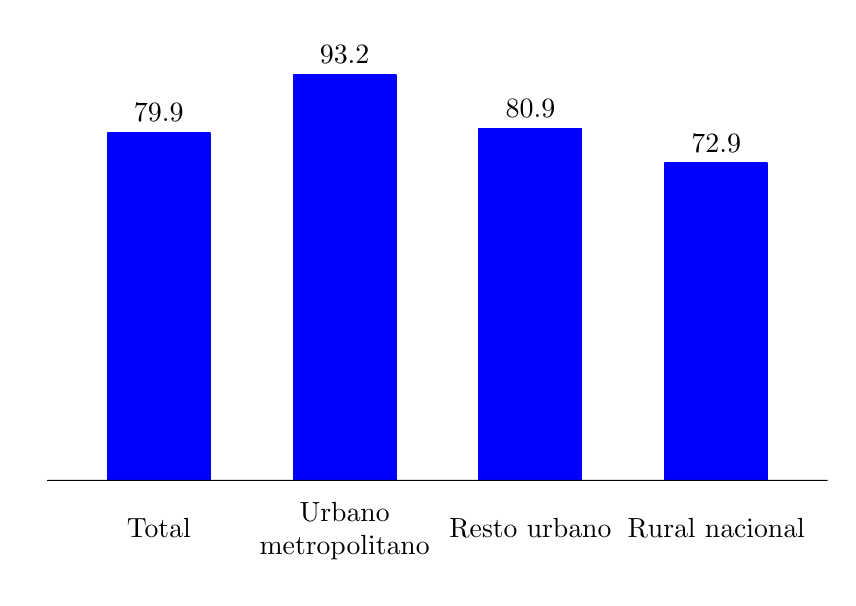
\begin{tikzpicture}[x=1pt,y=1pt]  % Created by tikzDevice version 0.7.0 on 2015-09-08 18:19:48
% !TEX encoding = UTF-8 Unicode
\definecolor[named]{fillColor}{rgb}{1.00,1.00,1.00}
\path[use as bounding box,fill=fillColor,fill opacity=0.00] (0,0) rectangle (289.08,198.74);
\begin{scope}
\path[clip] (  0.00,  0.00) rectangle (289.08,198.74);
\definecolor[named]{drawColor}{rgb}{1.00,1.00,1.00}

\path[draw=drawColor,line width= 0.6pt,line join=round,line cap=round] (  0.00,  0.00) rectangle (289.08,198.74);
\end{scope}
\begin{scope}
\path[clip] (  0.00,  0.00) rectangle (289.08,198.74);

\path[] (  7.11, 35.35) rectangle (289.08,181.67);

\path[] ( 47.39, 35.35) --
	( 47.39,181.67);

\path[] (114.53, 35.35) --
	(114.53,181.67);

\path[] (181.66, 35.35) --
	(181.66,181.67);

\path[] (248.80, 35.35) --
	(248.80,181.67);
\definecolor[named]{drawColor}{rgb}{0.00,0.00,1.00}
\definecolor[named]{fillColor}{rgb}{0.00,0.00,1.00}

\path[draw=drawColor,line width= 0.6pt,line join=round,fill=fillColor] ( 28.93, 35.35) rectangle ( 65.86,160.79);

\path[draw=drawColor,line width= 0.6pt,line join=round,fill=fillColor] ( 96.07, 35.35) rectangle (132.99,181.67);

\path[draw=drawColor,line width= 0.6pt,line join=round,fill=fillColor] (163.20, 35.35) rectangle (200.13,162.36);

\path[draw=drawColor,line width= 0.6pt,line join=round,fill=fillColor] (230.34, 35.35) rectangle (267.26,149.80);
\definecolor[named]{drawColor}{rgb}{0.00,0.00,0.00}
\definecolor[named]{fillColor}{rgb}{0.00,0.00,0.00}

\path[draw=drawColor,line width= 0.1pt,line join=round,fill=fillColor] (  7.11, 35.35) -- (289.08, 35.35);

\node[text=drawColor,anchor=base,inner sep=0pt, outer sep=0pt, scale=  1.01] at ( 47.39,164.75) {79.9};

\node[text=drawColor,anchor=base,inner sep=0pt, outer sep=0pt, scale=  1.01] at (114.53,185.63) {93.2};

\node[text=drawColor,anchor=base,inner sep=0pt, outer sep=0pt, scale=  1.01] at (181.66,166.32) {80.9};

\node[text=drawColor,anchor=base,inner sep=0pt, outer sep=0pt, scale=  1.01] at (248.80,153.76) {72.9};
\end{scope}
\begin{scope}
\path[clip] (  0.00,  0.00) rectangle (289.08,198.74);

\path[] (  7.11, 35.35) --
	(  7.11,181.67);
\end{scope}
\begin{scope}
\path[clip] (  0.00,  0.00) rectangle (289.08,198.74);

\path[] (  7.11, 35.35) --
	(289.08, 35.35);
\end{scope}
\begin{scope}
\path[clip] (  0.00,  0.00) rectangle (289.08,198.74);

\path[] ( 47.39, 31.08) --
	( 47.39, 35.35);

\path[] (114.53, 31.08) --
	(114.53, 35.35);

\path[] (181.66, 31.08) --
	(181.66, 35.35);

\path[] (248.80, 31.08) --
	(248.80, 35.35);
\end{scope}
\begin{scope}
\path[clip] (  0.00,  0.00) rectangle (289.08,198.74);
\definecolor[named]{drawColor}{rgb}{0.00,0.00,0.00}

\node[text=drawColor,anchor=base,inner sep=0pt, outer sep=0pt, scale=  1.00] at ( 47.39, 14.48) {Total};

\node[text=drawColor,anchor=base,inner sep=0pt, outer sep=0pt, scale=  1.00] at (114.53, 20.42) {Urbano };

\node[text=drawColor,anchor=base,inner sep=0pt, outer sep=0pt, scale=  1.00] at (114.53,  8.54) { metropolitano};

\node[text=drawColor,anchor=base,inner sep=0pt, outer sep=0pt, scale=  1.00] at (181.66, 14.48) {Resto urbano};

\node[text=drawColor,anchor=base,inner sep=0pt, outer sep=0pt, scale=  1.00] at (248.80, 14.48) {Rural nacional};
\end{scope}
  \end{tikzpicture}}{Instituto Nacional de Estadística, con datos de ENEI II-2013}

\cajita{PEA según nivel de escolaridad}{La distribución según el último nivel escolar aprobado por la población que es económicamente activa, muestra que el 40.7\% alcanzó hasta el nivel primario. Estudios superiores y de postgrado la tiene el 7.8\% de la PEA.
	
	 Otro indicador importante es que 19.4\% de la población económicamente activa, no ha obtenido ningún grado de escolaridad. }{Distribución de la población económicamente activa, según nivel de escolaridad}{República de Guatemala, año 2013, en porcentaje}{\ \\[0mm]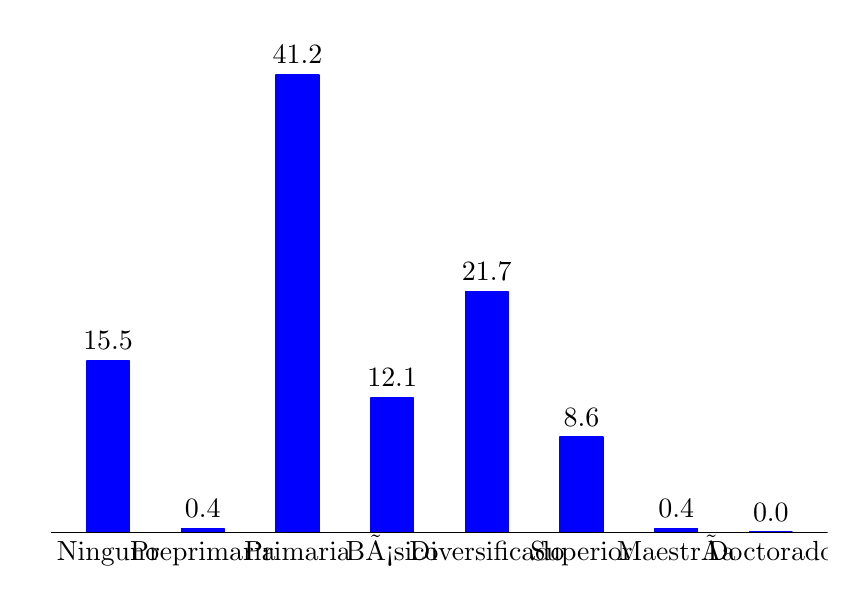
\begin{tikzpicture}[x=1pt,y=1pt]  % Created by tikzDevice version 0.9 on 2015-12-02 21:33:18
% !TEX encoding = UTF-8 Unicode
\definecolor{fillColor}{RGB}{255,255,255}
\path[use as bounding box,fill=fillColor,fill opacity=0.00] (0,0) rectangle (289.08,198.74);
\begin{scope}
\path[clip] (  0.00,  0.00) rectangle (289.08,198.74);

\path[] (  0.00,  0.00) rectangle (289.08,198.74);
\end{scope}
\begin{scope}
\path[clip] (  0.00,  0.00) rectangle (289.08,198.74);

\path[] (  8.54, 16.35) rectangle (289.08,181.67);

\path[] ( 29.06, 16.35) --
	( 29.06,181.67);

\path[] ( 63.28, 16.35) --
	( 63.28,181.67);

\path[] ( 97.49, 16.35) --
	( 97.49,181.67);

\path[] (131.70, 16.35) --
	(131.70,181.67);

\path[] (165.91, 16.35) --
	(165.91,181.67);

\path[] (200.13, 16.35) --
	(200.13,181.67);

\path[] (234.34, 16.35) --
	(234.34,181.67);

\path[] (268.55, 16.35) --
	(268.55,181.67);
\definecolor{drawColor}{RGB}{0,0,255}
\definecolor{fillColor}{RGB}{0,0,255}

\path[draw=drawColor,line width= 0.6pt,line join=round,fill=fillColor] ( 21.37, 16.35) rectangle ( 36.76, 78.40);

\path[draw=drawColor,line width= 0.6pt,line join=round,fill=fillColor] ( 55.58, 16.35) rectangle ( 70.97, 17.82);

\path[draw=drawColor,line width= 0.6pt,line join=round,fill=fillColor] ( 89.79, 16.35) rectangle (105.19,181.67);

\path[draw=drawColor,line width= 0.6pt,line join=round,fill=fillColor] (124.00, 16.35) rectangle (139.40, 64.98);

\path[draw=drawColor,line width= 0.6pt,line join=round,fill=fillColor] (158.22, 16.35) rectangle (173.61,103.45);

\path[draw=drawColor,line width= 0.6pt,line join=round,fill=fillColor] (192.43, 16.35) rectangle (207.82, 50.71);

\path[draw=drawColor,line width= 0.6pt,line join=round,fill=fillColor] (226.64, 16.35) rectangle (242.04, 17.78);

\path[draw=drawColor,line width= 0.6pt,line join=round,fill=fillColor] (260.85, 16.35) rectangle (276.25, 16.47);
\definecolor{drawColor}{RGB}{0,0,0}

\path[draw=drawColor,line width= 0.1pt,line join=round] (  8.54, 16.35) -- (289.08, 16.35);

\node[text=drawColor,anchor=base,inner sep=0pt, outer sep=0pt, scale=  1.01] at ( 29.06, 82.35) {15.5};

\node[text=drawColor,anchor=base,inner sep=0pt, outer sep=0pt, scale=  1.01] at ( 63.28, 21.77) {0.4};

\node[text=drawColor,anchor=base,inner sep=0pt, outer sep=0pt, scale=  1.01] at ( 97.49,185.63) {41.2};

\node[text=drawColor,anchor=base,inner sep=0pt, outer sep=0pt, scale=  1.01] at (131.70, 68.93) {12.1};

\node[text=drawColor,anchor=base,inner sep=0pt, outer sep=0pt, scale=  1.01] at (165.91,107.40) {21.7};

\node[text=drawColor,anchor=base,inner sep=0pt, outer sep=0pt, scale=  1.01] at (200.13, 54.67) {8.6};

\node[text=drawColor,anchor=base,inner sep=0pt, outer sep=0pt, scale=  1.01] at (234.34, 21.73) {0.4};

\node[text=drawColor,anchor=base,inner sep=0pt, outer sep=0pt, scale=  1.01] at (268.55, 20.43) {0.0};

\path[] (  8.54, 16.35) rectangle (289.08,181.67);
\end{scope}
\begin{scope}
\path[clip] (  0.00,  0.00) rectangle (289.08,198.74);

\path[] (  8.54, 16.35) --
	(  8.54,181.67);
\end{scope}
\begin{scope}
\path[clip] (  0.00,  0.00) rectangle (289.08,198.74);

\path[] (  8.54, 16.35) --
	(289.08, 16.35);
\end{scope}
\begin{scope}
\path[clip] (  0.00,  0.00) rectangle (289.08,198.74);

\path[] ( 29.06, 12.08) --
	( 29.06, 16.35);

\path[] ( 63.28, 12.08) --
	( 63.28, 16.35);

\path[] ( 97.49, 12.08) --
	( 97.49, 16.35);

\path[] (131.70, 12.08) --
	(131.70, 16.35);

\path[] (165.91, 12.08) --
	(165.91, 16.35);

\path[] (200.13, 12.08) --
	(200.13, 16.35);

\path[] (234.34, 12.08) --
	(234.34, 16.35);

\path[] (268.55, 12.08) --
	(268.55, 16.35);
\end{scope}
\begin{scope}
\path[clip] (  0.00,  0.00) rectangle (289.08,198.74);
\definecolor{drawColor}{RGB}{0,0,0}

\node[text=drawColor,anchor=base,inner sep=0pt, outer sep=0pt, scale=  1.00] at ( 29.06,  6.04) {Ninguno};

\node[text=drawColor,anchor=base,inner sep=0pt, outer sep=0pt, scale=  1.00] at ( 63.28,  6.04) {Preprimaria};

\node[text=drawColor,anchor=base,inner sep=0pt, outer sep=0pt, scale=  1.00] at ( 97.49,  6.04) {Primaria};

\node[text=drawColor,anchor=base,inner sep=0pt, outer sep=0pt, scale=  1.00] at (131.70,  6.04) {Básico};

\node[text=drawColor,anchor=base,inner sep=0pt, outer sep=0pt, scale=  1.00] at (165.91,  6.04) {Diversificado};

\node[text=drawColor,anchor=base,inner sep=0pt, outer sep=0pt, scale=  1.00] at (200.13,  6.04) {Superior};

\node[text=drawColor,anchor=base,inner sep=0pt, outer sep=0pt, scale=  1.00] at (234.34,  6.04) {Maestría};

\node[text=drawColor,anchor=base,inner sep=0pt, outer sep=0pt, scale=  1.00] at (268.55,  6.04) {Doctorado};
\end{scope}
  \end{tikzpicture}}{Instituto Nacional de Estadística, con datos de ENEI II-2013}



\cajita{PEA según escolaridad y sexo}{Las distribuciones de la población económicamente activa por hombre y mujer, muestra que ambos grupos tiene un mayor porcentaje con educación primaria.
	
	El 10.9\% de las mujeres que forman parte de la PEA tienen estudios superiores o de postgrado.}{Distribución de la población económicamente activa por sexo según nivel de escolaridad}{República de Guatemala, año 2013, en porcentaje}{\ \\[0mm]\begin{tikzpicture}[x=1pt,y=1pt]  % Created by tikzDevice version 0.9 on 2015-12-02 21:33:23
% !TEX encoding = UTF-8 Unicode
\definecolor{fillColor}{RGB}{255,255,255}
\path[use as bounding box,fill=fillColor,fill opacity=0.00] (0,0) rectangle (289.08,198.74);
\begin{scope}
\path[clip] (  0.00,  0.00) rectangle (289.08,198.74);

\path[] (  0.00,  0.00) rectangle (289.08,198.74);
\end{scope}
\begin{scope}
\path[clip] (  0.00,  0.00) rectangle (289.08,198.74);

\path[] (  7.11, 20.62) rectangle (289.08,172.85);

\path[] ( 30.61, 20.62) --
	( 30.61,172.85);

\path[] ( 69.77, 20.62) --
	( 69.77,172.85);

\path[] (108.93, 20.62) --
	(108.93,172.85);

\path[] (148.10, 20.62) --
	(148.10,172.85);

\path[] (187.26, 20.62) --
	(187.26,172.85);

\path[] (226.42, 20.62) --
	(226.42,172.85);

\path[] (265.58, 20.62) --
	(265.58,172.85);
\definecolor{drawColor}{RGB}{0,0,255}
\definecolor{fillColor}{RGB}{0,0,255}

\path[draw=drawColor,line width= 0.6pt,line join=round,fill=fillColor] ( 15.44, 20.62) rectangle ( 28.16, 71.37);
\definecolor{drawColor}{RGB}{157,187,255}
\definecolor{fillColor}{RGB}{157,187,255}

\path[draw=drawColor,line width= 0.6pt,line join=round,fill=fillColor] ( 33.06, 20.62) rectangle ( 45.79, 77.03);
\definecolor{drawColor}{RGB}{0,0,255}
\definecolor{fillColor}{RGB}{0,0,255}

\path[draw=drawColor,line width= 0.6pt,line join=round,fill=fillColor] ( 54.60, 20.62) rectangle ( 67.32, 21.74);
\definecolor{drawColor}{RGB}{157,187,255}
\definecolor{fillColor}{RGB}{157,187,255}

\path[draw=drawColor,line width= 0.6pt,line join=round,fill=fillColor] ( 72.22, 20.62) rectangle ( 84.95, 22.10);
\definecolor{drawColor}{RGB}{0,0,255}
\definecolor{fillColor}{RGB}{0,0,255}

\path[draw=drawColor,line width= 0.6pt,line join=round,fill=fillColor] ( 93.76, 20.62) rectangle (106.49,172.85);
\definecolor{drawColor}{RGB}{157,187,255}
\definecolor{fillColor}{RGB}{157,187,255}

\path[draw=drawColor,line width= 0.6pt,line join=round,fill=fillColor] (111.38, 20.62) rectangle (124.11,139.29);
\definecolor{drawColor}{RGB}{0,0,255}
\definecolor{fillColor}{RGB}{0,0,255}

\path[draw=drawColor,line width= 0.6pt,line join=round,fill=fillColor] (132.92, 20.62) rectangle (145.65, 65.23);
\definecolor{drawColor}{RGB}{157,187,255}
\definecolor{fillColor}{RGB}{157,187,255}

\path[draw=drawColor,line width= 0.6pt,line join=round,fill=fillColor] (150.54, 20.62) rectangle (163.27, 55.84);
\definecolor{drawColor}{RGB}{0,0,255}
\definecolor{fillColor}{RGB}{0,0,255}

\path[draw=drawColor,line width= 0.6pt,line join=round,fill=fillColor] (172.08, 20.62) rectangle (184.81, 86.45);
\definecolor{drawColor}{RGB}{157,187,255}
\definecolor{fillColor}{RGB}{157,187,255}

\path[draw=drawColor,line width= 0.6pt,line join=round,fill=fillColor] (189.71, 20.62) rectangle (202.43,109.86);
\definecolor{drawColor}{RGB}{0,0,255}
\definecolor{fillColor}{RGB}{0,0,255}

\path[draw=drawColor,line width= 0.6pt,line join=round,fill=fillColor] (211.25, 20.62) rectangle (223.97, 45.30);
\definecolor{drawColor}{RGB}{157,187,255}
\definecolor{fillColor}{RGB}{157,187,255}

\path[draw=drawColor,line width= 0.6pt,line join=round,fill=fillColor] (228.87, 20.62) rectangle (241.60, 58.22);
\definecolor{drawColor}{RGB}{0,0,255}
\definecolor{fillColor}{RGB}{0,0,255}

\path[draw=drawColor,line width= 0.6pt,line join=round,fill=fillColor] (250.41, 20.62) rectangle (263.14, 21.93);
\definecolor{drawColor}{RGB}{157,187,255}
\definecolor{fillColor}{RGB}{157,187,255}

\path[draw=drawColor,line width= 0.6pt,line join=round,fill=fillColor] (268.03, 20.62) rectangle (280.76, 21.94);
\definecolor{drawColor}{RGB}{0,0,0}

\path[draw=drawColor,line width= 0.6pt,line join=round] (  7.11, 20.62) -- (289.08, 20.62);

\node[text=drawColor,anchor=base,inner sep=0pt, outer sep=0pt, scale=  0.82] at ( 21.80, 74.59) {14.9};

\node[text=drawColor,anchor=base,inner sep=0pt, outer sep=0pt, scale=  0.82] at ( 39.42, 80.25) {16.5};

\node[text=drawColor,anchor=base,inner sep=0pt, outer sep=0pt, scale=  0.82] at ( 60.96, 24.96) {0.3};

\node[text=drawColor,anchor=base,inner sep=0pt, outer sep=0pt, scale=  0.82] at ( 78.58, 25.32) {0.4};

\node[text=drawColor,anchor=base,inner sep=0pt, outer sep=0pt, scale=  0.82] at (100.12,176.07) {44.6};

\node[text=drawColor,anchor=base,inner sep=0pt, outer sep=0pt, scale=  0.82] at (117.75,142.51) {34.8};

\node[text=drawColor,anchor=base,inner sep=0pt, outer sep=0pt, scale=  0.82] at (139.29, 68.45) {13.1};

\node[text=drawColor,anchor=base,inner sep=0pt, outer sep=0pt, scale=  0.82] at (156.91, 59.06) {10.3};

\node[text=drawColor,anchor=base,inner sep=0pt, outer sep=0pt, scale=  0.82] at (178.45, 89.67) {19.3};

\node[text=drawColor,anchor=base,inner sep=0pt, outer sep=0pt, scale=  0.82] at (196.07,113.08) {26.2};

\node[text=drawColor,anchor=base,inner sep=0pt, outer sep=0pt, scale=  0.82] at (217.61, 48.52) {7.2};

\node[text=drawColor,anchor=base,inner sep=0pt, outer sep=0pt, scale=  0.82] at (235.23, 61.44) {11.0};

\node[text=drawColor,anchor=base,inner sep=0pt, outer sep=0pt, scale=  0.82] at (256.77, 25.15) {0.4};

\node[text=drawColor,anchor=base,inner sep=0pt, outer sep=0pt, scale=  0.82] at (274.39, 25.17) {0.4};

\path[] (  7.11, 20.62) rectangle (289.08,172.85);
\end{scope}
\begin{scope}
\path[clip] (  0.00,  0.00) rectangle (289.08,198.74);

\path[] (  7.11, 20.62) --
	(  7.11,172.85);
\end{scope}
\begin{scope}
\path[clip] (  0.00,  0.00) rectangle (289.08,198.74);

\path[] (  7.11, 20.62) --
	(289.08, 20.62);
\end{scope}
\begin{scope}
\path[clip] (  0.00,  0.00) rectangle (289.08,198.74);

\path[] ( 30.61, 16.35) --
	( 30.61, 20.62);

\path[] ( 69.77, 16.35) --
	( 69.77, 20.62);

\path[] (108.93, 16.35) --
	(108.93, 20.62);

\path[] (148.10, 16.35) --
	(148.10, 20.62);

\path[] (187.26, 16.35) --
	(187.26, 20.62);

\path[] (226.42, 16.35) --
	(226.42, 20.62);

\path[] (265.58, 16.35) --
	(265.58, 20.62);
\end{scope}
\begin{scope}
\path[clip] (  0.00,  0.00) rectangle (289.08,198.74);
\definecolor{drawColor}{RGB}{0,0,0}

\node[text=drawColor,anchor=base,inner sep=0pt, outer sep=0pt, scale=  1.00] at ( 30.61,  5.69) {Ninguno};

\node[text=drawColor,anchor=base,inner sep=0pt, outer sep=0pt, scale=  1.00] at ( 69.77,  5.69) {Preprimaria};

\node[text=drawColor,anchor=base,inner sep=0pt, outer sep=0pt, scale=  1.00] at (108.93,  5.69) {Primaria};

\node[text=drawColor,anchor=base,inner sep=0pt, outer sep=0pt, scale=  1.00] at (148.10,  5.69) {Básico};

\node[text=drawColor,anchor=base,inner sep=0pt, outer sep=0pt, scale=  1.00] at (187.26,  5.69) {Diversificado};

\node[text=drawColor,anchor=base,inner sep=0pt, outer sep=0pt, scale=  1.00] at (226.42,  5.69) {Superior};

\node[text=drawColor,anchor=base,inner sep=0pt, outer sep=0pt, scale=  1.00] at (265.58,  5.69) {Postgrado};
\end{scope}
\begin{scope}
\path[clip] (  0.00,  0.00) rectangle (289.08,198.74);
\coordinate (apoyo) at (55.98,189.21);
\coordinate (longitudFicticia) at (7.11,9.53);
\coordinate (longitud) at (7.11,7.11);
\coordinate (desX) at (142.21,0);
\coordinate (desY) at (0,1.21);
\definecolor[named]{ct1}{HTML}{
0000FF
}
\definecolor[named]{ct2}{HTML}{
9DBBFF
}
\definecolor[named]{ctb1}{HTML}{
0000FF
}
\definecolor[named]{ctb2}{HTML}{
9DBBFF
}
\path [fill=none] (apoyo) rectangle ($(apoyo)+(longitudFicticia)$)
node [xshift=0.3cm,inner sep=0pt, outer sep=0pt,midway,right,scale = 0.9]{Hombre};
\draw [color = ctb1,fill=ct1] ( $(apoyo)  + (desY) $) rectangle ($(apoyo)+ (desY) +(longitud)$);
\path [fill=none] ($(apoyo)+(desX)$) rectangle ($(apoyo)+(desX)+(longitudFicticia)$)
node [xshift=0.3cm,inner sep=0pt, outer sep=0pt,midway,right,scale = 0.9]{Mujer};
\draw [color = ctb2 ,fill=ct2] ( $(apoyo)  + (desY) + (desX) $) rectangle ($(apoyo)+ (desY)+ (desX) +(longitud)$);
\end{scope}
  \end{tikzpicture}}{Instituto Nacional de Estadística, con datos de ENEI II-2013}

\cajita{PEA según escolaridad y etnia}{Las distribuciones de la población económicamente activa  por grupo ético, muestra que ambos grupos tiene un mayor porcentaje con educación primaria.
	
	El 11.4\% de la población no indígena que forma parte de la PEA tiene estudios superiores o de postgrado.
	
	El 29.3 de la PEA con etnicidad indígena no tiene ningún nivel de escolaridad aprobado.}{Distribución de la población económicamente activa por grupo étnico según nivel de escolaridad}{República de Guatemala, año 2013, en porcentaje}{\ \\[0mm]\begin{tikzpicture}[x=1pt,y=1pt]  % Created by tikzDevice version 0.7.0 on 2015-08-28 14:06:57
% !TEX encoding = UTF-8 Unicode
\definecolor[named]{fillColor}{rgb}{1.00,1.00,1.00}
\path[use as bounding box,fill=fillColor,fill opacity=0.00] (0,0) rectangle (289.08,198.74);
\begin{scope}
\path[clip] (  0.00,  0.00) rectangle (289.08,198.74);
\definecolor[named]{drawColor}{rgb}{1.00,1.00,1.00}

\path[draw=drawColor,line width= 0.6pt,line join=round,line cap=round] (  0.00,  0.00) rectangle (289.08,198.74);
\end{scope}
\begin{scope}
\path[clip] (  0.00,  0.00) rectangle (289.08,198.74);

\path[] (  7.11, 20.62) rectangle (289.08,172.42);

\path[] ( 34.40, 20.62) --
	( 34.40,172.42);

\path[] ( 79.88, 20.62) --
	( 79.88,172.42);

\path[] (125.36, 20.62) --
	(125.36,172.42);

\path[] (170.84, 20.62) --
	(170.84,172.42);

\path[] (216.31, 20.62) --
	(216.31,172.42);

\path[] (261.79, 20.62) --
	(261.79,172.42);
\definecolor[named]{drawColor}{rgb}{0.00,0.00,1.00}
\definecolor[named]{fillColor}{rgb}{0.00,0.00,1.00}

\path[draw=drawColor,line width= 0.6pt,line join=round,fill=fillColor] ( 16.78, 20.62) rectangle ( 31.56, 61.32);
\definecolor[named]{drawColor}{rgb}{0.62,0.73,1.00}
\definecolor[named]{fillColor}{rgb}{0.62,0.73,1.00}

\path[draw=drawColor,line width= 0.6pt,line join=round,fill=fillColor] ( 37.24, 20.62) rectangle ( 52.02,115.26);
\definecolor[named]{drawColor}{rgb}{0.00,0.00,1.00}
\definecolor[named]{fillColor}{rgb}{0.00,0.00,1.00}

\path[draw=drawColor,line width= 0.6pt,line join=round,fill=fillColor] ( 62.26, 20.62) rectangle ( 77.04,138.19);
\definecolor[named]{drawColor}{rgb}{0.62,0.73,1.00}
\definecolor[named]{fillColor}{rgb}{0.62,0.73,1.00}

\path[draw=drawColor,line width= 0.6pt,line join=round,fill=fillColor] ( 82.72, 20.62) rectangle ( 97.50,172.42);
\definecolor[named]{drawColor}{rgb}{0.00,0.00,1.00}
\definecolor[named]{fillColor}{rgb}{0.00,0.00,1.00}

\path[draw=drawColor,line width= 0.6pt,line join=round,fill=fillColor] (107.73, 20.62) rectangle (122.51, 71.65);
\definecolor[named]{drawColor}{rgb}{0.62,0.73,1.00}
\definecolor[named]{fillColor}{rgb}{0.62,0.73,1.00}

\path[draw=drawColor,line width= 0.6pt,line join=round,fill=fillColor] (128.20, 20.62) rectangle (142.98, 53.24);
\definecolor[named]{drawColor}{rgb}{0.00,0.00,1.00}
\definecolor[named]{fillColor}{rgb}{0.00,0.00,1.00}

\path[draw=drawColor,line width= 0.6pt,line join=round,fill=fillColor] (153.21, 20.62) rectangle (167.99, 97.81);
\definecolor[named]{drawColor}{rgb}{0.62,0.73,1.00}
\definecolor[named]{fillColor}{rgb}{0.62,0.73,1.00}

\path[draw=drawColor,line width= 0.6pt,line join=round,fill=fillColor] (173.68, 20.62) rectangle (188.46, 56.15);
\definecolor[named]{drawColor}{rgb}{0.00,0.00,1.00}
\definecolor[named]{fillColor}{rgb}{0.00,0.00,1.00}

\path[draw=drawColor,line width= 0.6pt,line join=round,fill=fillColor] (198.69, 20.62) rectangle (213.47, 54.86);
\definecolor[named]{drawColor}{rgb}{0.62,0.73,1.00}
\definecolor[named]{fillColor}{rgb}{0.62,0.73,1.00}

\path[draw=drawColor,line width= 0.6pt,line join=round,fill=fillColor] (219.16, 20.62) rectangle (233.94, 28.70);
\definecolor[named]{drawColor}{rgb}{0.00,0.00,1.00}
\definecolor[named]{fillColor}{rgb}{0.00,0.00,1.00}

\path[draw=drawColor,line width= 0.6pt,line join=round,fill=fillColor] (244.17, 20.62) rectangle (258.95, 23.20);
\definecolor[named]{drawColor}{rgb}{0.62,0.73,1.00}
\definecolor[named]{fillColor}{rgb}{0.62,0.73,1.00}

\path[draw=drawColor,line width= 0.6pt,line join=round,fill=fillColor] (264.64, 20.62) rectangle (279.42, 20.94);
\definecolor[named]{drawColor}{rgb}{0.00,0.00,0.00}
\definecolor[named]{fillColor}{rgb}{0.00,0.00,0.00}

\path[draw=drawColor,line width= 0.6pt,line join=round,fill=fillColor] (  7.11, 20.62) -- (289.08, 20.62);

\node[text=drawColor,anchor=base,inner sep=0pt, outer sep=0pt, scale=  0.82] at ( 24.17, 64.54) {12.6};

\node[text=drawColor,anchor=base,inner sep=0pt, outer sep=0pt, scale=  0.82] at ( 44.63,118.48) {29.3};

\node[text=drawColor,anchor=base,inner sep=0pt, outer sep=0pt, scale=  0.82] at ( 69.65,141.41) {36.4};

\node[text=drawColor,anchor=base,inner sep=0pt, outer sep=0pt, scale=  0.82] at ( 90.11,175.65) {47.0};

\node[text=drawColor,anchor=base,inner sep=0pt, outer sep=0pt, scale=  0.82] at (115.12, 74.88) {15.8};

\node[text=drawColor,anchor=base,inner sep=0pt, outer sep=0pt, scale=  0.82] at (135.59, 56.47) {10.1};

\node[text=drawColor,anchor=base,inner sep=0pt, outer sep=0pt, scale=  0.82] at (160.60,101.04) {23.9};

\node[text=drawColor,anchor=base,inner sep=0pt, outer sep=0pt, scale=  0.82] at (181.07, 59.37) {11.0};

\node[text=drawColor,anchor=base,inner sep=0pt, outer sep=0pt, scale=  0.82] at (206.08, 58.08) {10.6};

\node[text=drawColor,anchor=base,inner sep=0pt, outer sep=0pt, scale=  0.82] at (226.55, 31.92) {2.5};

\node[text=drawColor,anchor=base,inner sep=0pt, outer sep=0pt, scale=  0.82] at (251.56, 26.43) {0.8};

\node[text=drawColor,anchor=base,inner sep=0pt, outer sep=0pt, scale=  0.82] at (272.03, 24.17) {0.1};
\end{scope}
\begin{scope}
\path[clip] (  0.00,  0.00) rectangle (289.08,198.74);

\path[] (  7.11, 20.62) --
	(  7.11,172.42);
\end{scope}
\begin{scope}
\path[clip] (  0.00,  0.00) rectangle (289.08,198.74);

\path[] (  7.11, 20.62) --
	(289.08, 20.62);
\end{scope}
\begin{scope}
\path[clip] (  0.00,  0.00) rectangle (289.08,198.74);

\path[] ( 34.40, 16.35) --
	( 34.40, 20.62);

\path[] ( 79.88, 16.35) --
	( 79.88, 20.62);

\path[] (125.36, 16.35) --
	(125.36, 20.62);

\path[] (170.84, 16.35) --
	(170.84, 20.62);

\path[] (216.31, 16.35) --
	(216.31, 20.62);

\path[] (261.79, 16.35) --
	(261.79, 20.62);
\end{scope}
\begin{scope}
\path[clip] (  0.00,  0.00) rectangle (289.08,198.74);
\definecolor[named]{drawColor}{rgb}{0.00,0.00,0.00}

\node[text=drawColor,anchor=base,inner sep=0pt, outer sep=0pt, scale=  1.00] at ( 34.40,  5.69) {Ninguno};

\node[text=drawColor,anchor=base,inner sep=0pt, outer sep=0pt, scale=  1.00] at ( 79.88,  5.69) {Primaria};

\node[text=drawColor,anchor=base,inner sep=0pt, outer sep=0pt, scale=  1.00] at (125.36,  5.69) {B\'asico};

\node[text=drawColor,anchor=base,inner sep=0pt, outer sep=0pt, scale=  1.00] at (170.84,  5.69) {Diversificado};

\node[text=drawColor,anchor=base,inner sep=0pt, outer sep=0pt, scale=  1.00] at (216.31,  5.69) {Superior};

\node[text=drawColor,anchor=base,inner sep=0pt, outer sep=0pt, scale=  1.00] at (261.79,  5.69) {Postgrado};
\end{scope}
\coordinate (apoyo) at (49.65,188.79);
\coordinate (longitudFicticia) at (7.11,9.95);
\coordinate (longitud) at (7.11,7.11);
\coordinate (desX) at (144.31,0);
\coordinate (desY) at (0,1.42);
\definecolor[named]{ct1}{HTML}{
0000FF
}
\definecolor[named]{ct2}{HTML}{
9DBBFF
}
\definecolor[named]{ctb1}{HTML}{
0000FF
}
\definecolor[named]{ctb2}{HTML}{
9DBBFF
}
\path [fill=none] (apoyo) rectangle ($(apoyo)+(longitudFicticia)$)
node [xshift=0.3cm,inner sep=0pt, outer sep=0pt,midway,right,scale = 0.9]{No ind\'igena};
\draw [color = ctb1,fill=ct1] ( $(apoyo)  + (desY) $) rectangle ($(apoyo)+ (desY) +(longitud)$);
\path [fill=none] ($(apoyo)+(desX)$) rectangle ($(apoyo)+(desX)+(longitudFicticia)$)
node [xshift=0.3cm,inner sep=0pt, outer sep=0pt,midway,right,scale = 0.9]{Ind\'igena};
\draw [color = ctb2 ,fill=ct2] ( $(apoyo)  + (desY) + (desX) $) rectangle ($(apoyo)+ (desY)+ (desX) +(longitud)$);
  \end{tikzpicture}}{Instituto Nacional de Estadística, con datos de ENEI II-2013}


\cajita{PEA que asistió a un plantel educativo}{De la población económicamente activa, el 90.3\% asistió, en el 2013, a un plantel educativo.}{Distribución de la población económicamente activa, de acuerdo a su asistencia a un plantel educativo}{República de Guatemala, año 2013, en porcentaje}{\ \\[0mm]\begin{tikzpicture}[x=1pt,y=1pt]  % Created by tikzDevice version 0.7.0 on 2015-08-31 18:57:46
% !TEX encoding = UTF-8 Unicode
\definecolor[named]{fillColor}{rgb}{1.00,1.00,1.00}
\path[use as bounding box,fill=fillColor,fill opacity=0.00] (0,0) rectangle (289.08,198.74);
\begin{scope}
\path[clip] ( 30.54,  0.00) rectangle (258.54,198.74);
\definecolor[named]{drawColor}{rgb}{1.00,1.00,1.00}

\path[draw=drawColor,line width= 0.6pt,line join=round,line cap=round] ( 30.54,  0.00) rectangle (258.54,198.74);
\end{scope}
\begin{scope}
\path[clip] (  0.00,  0.00) rectangle (289.08,198.74);

\path[] (  9.28,  7.11) rectangle (200.91,198.74);

\path[] (105.09,102.93) --
	(130.96, 20.67);

\path[] (105.09,102.93) --
	( 79.22,185.19);

\path[] (105.09,102.93) --
	(187.35,128.80);

\path[] (105.09,102.93) --
	(130.96, 20.67);

\path[] (105.09,102.93) --
	( 22.83, 77.05);

\path[] (105.09,102.93) --
	( 79.22,185.19);

\path[] (105.09,102.93) --
	(105.09,102.93) --
	(105.09,102.93) --
	(105.09,102.93) --
	(105.09,102.93) --
	(105.09,102.93) --
	(105.09,102.93) --
	(105.09,102.93) --
	(105.09,102.93) --
	(105.09,102.93) --
	(105.09,102.93) --
	(105.09,102.93) --
	(105.09,102.93) --
	(105.09,102.93) --
	(105.09,102.93) --
	(105.09,102.93) --
	(105.09,102.93) --
	(105.09,102.93) --
	(105.09,102.93) --
	(105.09,102.93) --
	(105.09,102.93) --
	(105.09,102.93) --
	(105.09,102.93) --
	(105.09,102.93) --
	(105.09,102.93) --
	(105.09,102.93) --
	(105.09,102.93) --
	(105.09,102.93) --
	(105.09,102.93) --
	(105.09,102.93) --
	(105.09,102.93) --
	(105.09,102.93) --
	(105.09,102.93) --
	(105.09,102.93) --
	(105.09,102.93) --
	(105.09,102.93) --
	(105.09,102.93) --
	(105.09,102.93) --
	(105.09,102.93) --
	(105.09,102.93) --
	(105.09,102.93) --
	(105.09,102.93) --
	(105.09,102.93) --
	(105.09,102.93) --
	(105.09,102.93) --
	(105.09,102.93) --
	(105.09,102.93) --
	(105.09,102.93) --
	(105.09,102.93) --
	(105.09,102.93) --
	(105.09,102.93) --
	(105.09,102.93) --
	(105.09,102.93) --
	(105.09,102.93) --
	(105.09,102.93) --
	(105.09,102.93) --
	(105.09,102.93) --
	(105.09,102.93) --
	(105.09,102.93) --
	(105.09,102.93) --
	(105.09,102.93) --
	(105.09,102.93) --
	(105.09,102.93) --
	(105.09,102.93) --
	(105.09,102.93) --
	(105.09,102.93) --
	(105.09,102.93) --
	(105.09,102.93) --
	(105.09,102.93) --
	(105.09,102.93) --
	(105.09,102.93) --
	(105.09,102.93) --
	(105.09,102.93) --
	(105.09,102.93) --
	(105.09,102.93) --
	(105.09,102.93) --
	(105.09,102.93) --
	(105.09,102.93) --
	(105.09,102.93) --
	(105.09,102.93) --
	(105.09,102.93) --
	(105.09,102.93) --
	(105.09,102.93) --
	(105.09,102.93) --
	(105.09,102.93) --
	(105.09,102.93) --
	(105.09,102.93) --
	(105.09,102.93) --
	(105.09,102.93) --
	(105.09,102.93) --
	(105.09,102.93) --
	(105.09,102.93) --
	(105.09,102.93) --
	(105.09,102.93) --
	(105.09,102.93) --
	(105.09,102.93) --
	(105.09,102.93) --
	(105.09,102.93) --
	(105.09,102.93) --
	(105.09,102.93);

\path[] (105.09,122.09) --
	(106.31,122.05) --
	(107.52,121.94) --
	(108.72,121.74) --
	(109.90,121.48) --
	(111.07,121.13) --
	(112.21,120.72) --
	(113.33,120.23) --
	(114.41,119.67) --
	(115.45,119.05) --
	(116.45,118.36) --
	(117.41,117.61) --
	(118.32,116.80) --
	(119.17,115.93) --
	(119.96,115.01) --
	(120.70,114.04) --
	(121.37,113.03) --
	(121.98,111.98) --
	(122.52,110.89) --
	(122.99,109.77) --
	(123.39,108.62) --
	(123.71,107.45) --
	(123.96,106.26) --
	(124.14,105.05) --
	(124.23,103.84) --
	(124.25,102.62) --
	(124.19,101.41) --
	(124.06,100.20) --
	(123.85, 99.00) --
	(123.56, 97.82) --
	(123.20, 96.66) --
	(122.77, 95.52) --
	(122.26, 94.42) --
	(121.69, 93.35) --
	(121.05, 92.31) --
	(120.34, 91.32) --
	(119.57, 90.38) --
	(118.75, 89.49) --
	(117.87, 88.65) --
	(116.94, 87.86) --
	(115.96, 87.14) --
	(114.93, 86.49) --
	(113.87, 85.90) --
	(112.77, 85.37) --
	(111.65, 84.92) --
	(110.49, 84.54) --
	(109.31, 84.24) --
	(108.12, 84.01) --
	(106.91, 83.85) --
	(105.70, 83.77) --
	(104.48, 83.77) --
	(103.27, 83.85) --
	(102.06, 84.01) --
	(100.87, 84.24) --
	( 99.69, 84.54) --
	( 98.54, 84.92) --
	( 97.41, 85.37) --
	( 96.31, 85.90) --
	( 95.25, 86.49) --
	( 94.22, 87.14) --
	( 93.25, 87.86) --
	( 92.31, 88.65) --
	( 91.43, 89.49) --
	( 90.61, 90.38) --
	( 89.84, 91.32) --
	( 89.14, 92.31) --
	( 88.50, 93.35) --
	( 87.92, 94.42) --
	( 87.42, 95.52) --
	( 86.98, 96.66) --
	( 86.62, 97.82) --
	( 86.33, 99.00) --
	( 86.12,100.20) --
	( 85.99,101.41) --
	( 85.93,102.62) --
	( 85.95,103.84) --
	( 86.05,105.05) --
	( 86.22,106.26) --
	( 86.47,107.45) --
	( 86.79,108.62) --
	( 87.19,109.77) --
	( 87.66,110.89) --
	( 88.20,111.98) --
	( 88.81,113.03) --
	( 89.48,114.04) --
	( 90.22,115.01) --
	( 91.01,115.93) --
	( 91.87,116.80) --
	( 92.77,117.61) --
	( 93.73,118.36) --
	( 94.73,119.05) --
	( 95.77,119.67) --
	( 96.85,120.23) --
	( 97.97,120.72) --
	( 99.11,121.13) --
	(100.28,121.48) --
	(101.46,121.74) --
	(102.67,121.94) --
	(103.88,122.05) --
	(105.09,122.09);

\path[] (105.09,141.25) --
	(107.52,141.18) --
	(109.94,140.95) --
	(112.34,140.56) --
	(114.72,140.03) --
	(117.05,139.34) --
	(119.34,138.51) --
	(121.56,137.53) --
	(123.72,136.42) --
	(125.81,135.17) --
	(127.81,133.79) --
	(129.73,132.29) --
	(131.54,130.67) --
	(133.24,128.93) --
	(134.84,127.09) --
	(136.31,125.16) --
	(137.66,123.13) --
	(138.87,121.03) --
	(139.95,118.85) --
	(140.89,116.61) --
	(141.69,114.31) --
	(142.34,111.96) --
	(142.83,109.58) --
	(143.18,107.18) --
	(143.37,104.75) --
	(143.41,102.32) --
	(143.30, 99.89) --
	(143.03, 97.47) --
	(142.60, 95.08) --
	(142.03, 92.72) --
	(141.31, 90.39) --
	(140.44, 88.12) --
	(139.43, 85.91) --
	(138.28, 83.76) --
	(137.00, 81.70) --
	(135.59, 79.72) --
	(134.06, 77.83) --
	(132.41, 76.04) --
	(130.65, 74.36) --
	(128.78, 72.80) --
	(126.82, 71.36) --
	(124.78, 70.04) --
	(122.65, 68.86) --
	(120.46, 67.82) --
	(118.20, 66.91) --
	(115.89, 66.15) --
	(113.53, 65.54) --
	(111.15, 65.08) --
	(108.73, 64.78) --
	(106.31, 64.62) --
	(103.88, 64.62) --
	(101.45, 64.78) --
	( 99.04, 65.08) --
	( 96.65, 65.54) --
	( 94.29, 66.15) --
	( 91.98, 66.91) --
	( 89.73, 67.82) --
	( 87.53, 68.86) --
	( 85.40, 70.04) --
	( 83.36, 71.36) --
	( 81.40, 72.80) --
	( 79.54, 74.36) --
	( 77.78, 76.04) --
	( 76.13, 77.83) --
	( 74.59, 79.72) --
	( 73.18, 81.70) --
	( 71.90, 83.76) --
	( 70.75, 85.91) --
	( 69.74, 88.12) --
	( 68.87, 90.39) --
	( 68.15, 92.72) --
	( 67.58, 95.08) --
	( 67.16, 97.47) --
	( 66.89, 99.89) --
	( 66.77,102.32) --
	( 66.81,104.75) --
	( 67.00,107.18) --
	( 67.35,109.58) --
	( 67.85,111.96) --
	( 68.49,114.31) --
	( 69.29,116.61) --
	( 70.23,118.85) --
	( 71.31,121.03) --
	( 72.52,123.13) --
	( 73.87,125.16) --
	( 75.34,127.09) --
	( 76.94,128.93) --
	( 78.64,130.67) --
	( 80.46,132.29) --
	( 82.37,133.79) --
	( 84.37,135.17) --
	( 86.46,136.42) --
	( 88.62,137.53) --
	( 90.85,138.51) --
	( 93.13,139.34) --
	( 95.47,140.03) --
	( 97.84,140.56) --
	(100.24,140.95) --
	(102.66,141.18) --
	(105.09,141.25);

\path[] (105.09,160.42) --
	(108.74,160.30) --
	(112.37,159.95) --
	(115.97,159.38) --
	(119.53,158.57) --
	(123.03,157.55) --
	(126.46,156.30) --
	(129.80,154.84) --
	(133.04,153.16) --
	(136.17,151.29) --
	(139.18,149.22) --
	(142.04,146.97) --
	(144.76,144.53) --
	(147.32,141.93) --
	(149.71,139.18) --
	(151.92,136.27) --
	(153.94,133.24) --
	(155.76,130.08) --
	(157.38,126.81) --
	(158.79,123.44) --
	(159.99,120.00) --
	(160.96,116.48) --
	(161.71,112.91) --
	(162.23,109.30) --
	(162.51,105.66) --
	(162.57,102.02) --
	(162.40, 98.37) --
	(161.99, 94.75) --
	(161.36, 91.15) --
	(160.50, 87.61) --
	(159.42, 84.13) --
	(158.12, 80.72) --
	(156.60, 77.40) --
	(154.88, 74.18) --
	(152.95, 71.08) --
	(150.84, 68.11) --
	(148.54, 65.28) --
	(146.06, 62.60) --
	(143.42, 60.08) --
	(140.63, 57.74) --
	(137.69, 55.58) --
	(134.62, 53.60) --
	(131.43, 51.83) --
	(128.14, 50.26) --
	(124.75, 48.91) --
	(121.29, 47.77) --
	(117.76, 46.85) --
	(114.17, 46.16) --
	(110.56, 45.70) --
	(106.92, 45.47) --
	(103.27, 45.47) --
	( 99.63, 45.70) --
	( 96.01, 46.16) --
	( 92.43, 46.85) --
	( 88.89, 47.77) --
	( 85.43, 48.91) --
	( 82.04, 50.26) --
	( 78.75, 51.83) --
	( 75.56, 53.60) --
	( 72.49, 55.58) --
	( 69.55, 57.74) --
	( 66.76, 60.08) --
	( 64.12, 62.60) --
	( 61.64, 65.28) --
	( 59.34, 68.11) --
	( 57.23, 71.08) --
	( 55.30, 74.18) --
	( 53.58, 77.40) --
	( 52.07, 80.72) --
	( 50.76, 84.13) --
	( 49.68, 87.61) --
	( 48.82, 91.15) --
	( 48.19, 94.75) --
	( 47.78, 98.37) --
	( 47.61,102.02) --
	( 47.67,105.66) --
	( 47.96,109.30) --
	( 48.48,112.91) --
	( 49.22,116.48) --
	( 50.19,120.00) --
	( 51.39,123.44) --
	( 52.80,126.81) --
	( 54.42,130.08) --
	( 56.24,133.24) --
	( 58.26,136.27) --
	( 60.47,139.18) --
	( 62.86,141.93) --
	( 65.42,144.53) --
	( 68.14,146.97) --
	( 71.01,149.22) --
	( 74.01,151.29) --
	( 77.14,153.16) --
	( 80.38,154.84) --
	( 83.72,156.30) --
	( 87.15,157.55) --
	( 90.65,158.57) --
	( 94.21,159.38) --
	( 97.81,159.95) --
	(101.44,160.30) --
	(105.09,160.42);

\path[] (105.09,179.58) --
	(109.95,179.43) --
	(114.79,178.96) --
	(119.60,178.19) --
	(124.34,177.12) --
	(129.01,175.75) --
	(133.58,174.09) --
	(138.04,172.14) --
	(142.36,169.91) --
	(146.53,167.41) --
	(150.54,164.65) --
	(154.36,161.65) --
	(157.99,158.40) --
	(161.40,154.94) --
	(164.58,151.26) --
	(167.53,147.39) --
	(170.22,143.34) --
	(172.66,139.13) --
	(174.82,134.77) --
	(176.70,130.28) --
	(178.29,125.69) --
	(179.58,121.00) --
	(180.58,116.24) --
	(181.27,111.42) --
	(181.66,106.58) --
	(181.73,101.71) --
	(181.50, 96.85) --
	(180.96, 92.02) --
	(180.12, 87.23) --
	(178.97, 82.50) --
	(177.53, 77.86) --
	(175.79, 73.31) --
	(173.77, 68.89) --
	(171.47, 64.60) --
	(168.91, 60.47) --
	(166.09, 56.51) --
	(163.02, 52.73) --
	(159.72, 49.16) --
	(156.20, 45.80) --
	(152.47, 42.68) --
	(148.56, 39.79) --
	(144.47, 37.16) --
	(140.21, 34.80) --
	(135.82, 32.71) --
	(131.31, 30.90) --
	(126.69, 29.38) --
	(121.98, 28.16) --
	(117.20, 27.24) --
	(112.38, 26.62) --
	(107.52, 26.31) --
	(102.66, 26.31) --
	( 97.80, 26.62) --
	( 92.98, 27.24) --
	( 88.20, 28.16) --
	( 83.50, 29.38) --
	( 78.87, 30.90) --
	( 74.36, 32.71) --
	( 69.97, 34.80) --
	( 65.72, 37.16) --
	( 61.62, 39.79) --
	( 57.71, 42.68) --
	( 53.98, 45.80) --
	( 50.46, 49.16) --
	( 47.16, 52.73) --
	( 44.09, 56.51) --
	( 41.27, 60.47) --
	( 38.71, 64.60) --
	( 36.41, 68.89) --
	( 34.39, 73.31) --
	( 32.66, 77.86) --
	( 31.21, 82.50) --
	( 30.06, 87.23) --
	( 29.22, 92.02) --
	( 28.68, 96.85) --
	( 28.45,101.71) --
	( 28.53,106.58) --
	( 28.91,111.42) --
	( 29.60,116.24) --
	( 30.60,121.00) --
	( 31.90,125.69) --
	( 33.49,130.28) --
	( 35.37,134.77) --
	( 37.53,139.13) --
	( 39.96,143.34) --
	( 42.65,147.39) --
	( 45.60,151.26) --
	( 48.78,154.94) --
	( 52.20,158.40) --
	( 55.82,161.65) --
	( 59.64,164.65) --
	( 63.65,167.41) --
	( 67.82,169.91) --
	( 72.15,172.14) --
	( 76.60,174.09) --
	( 81.17,175.75) --
	( 85.84,177.12) --
	( 90.58,178.19) --
	( 95.39,178.96) --
	(100.23,179.43) --
	(105.09,179.58);

\path[] (105.09,189.16) --
	(110.56,188.99) --
	(116.01,188.47) --
	(121.41,187.60) --
	(126.75,186.40) --
	(132.00,184.86) --
	(137.14,182.98) --
	(142.15,180.79) --
	(147.02,178.28) --
	(151.71,175.47) --
	(156.22,172.37) --
	(160.52,168.99) --
	(164.60,165.34) --
	(168.44,161.44) --
	(172.02,157.30) --
	(175.33,152.95) --
	(178.37,148.39) --
	(181.10,143.65) --
	(183.53,138.75) --
	(185.65,133.70) --
	(187.44,128.53) --
	(188.89,123.26) --
	(190.01,117.90) --
	(190.79,112.49) --
	(191.23,107.03) --
	(191.31,101.56) --
	(191.05, 96.09) --
	(190.45, 90.66) --
	(189.50, 85.27) --
	(188.21, 79.95) --
	(186.58, 74.72) --
	(184.63, 69.61) --
	(182.36, 64.63) --
	(179.77, 59.81) --
	(176.89, 55.16) --
	(173.71, 50.70) --
	(170.26, 46.46) --
	(166.55, 42.44) --
	(162.59, 38.66) --
	(158.40, 35.14) --
	(153.99, 31.90) --
	(149.39, 28.94) --
	(144.61, 26.28) --
	(139.66, 23.93) --
	(134.58, 21.90) --
	(129.39, 20.19) --
	(124.09, 18.81) --
	(118.72, 17.78) --
	(113.29, 17.09) --
	(107.83, 16.74) --
	(102.36, 16.74) --
	( 96.89, 17.09) --
	( 91.47, 17.78) --
	( 86.09, 18.81) --
	( 80.80, 20.19) --
	( 75.60, 21.90) --
	( 70.52, 23.93) --
	( 65.58, 26.28) --
	( 60.80, 28.94) --
	( 56.19, 31.90) --
	( 51.79, 35.14) --
	( 47.59, 38.66) --
	( 43.63, 42.44) --
	( 39.92, 46.46) --
	( 36.47, 50.70) --
	( 33.30, 55.16) --
	( 30.41, 59.81) --
	( 27.83, 64.63) --
	( 25.55, 69.61) --
	( 23.60, 74.72) --
	( 21.98, 79.95) --
	( 20.69, 85.27) --
	( 19.74, 90.66) --
	( 19.13, 96.09) --
	( 18.87,101.56) --
	( 18.96,107.03) --
	( 19.39,112.49) --
	( 20.17,117.90) --
	( 21.29,123.26) --
	( 22.75,128.53) --
	( 24.54,133.70) --
	( 26.65,138.75) --
	( 29.08,143.65) --
	( 31.82,148.39) --
	( 34.85,152.95) --
	( 38.16,157.30) --
	( 41.74,161.44) --
	( 45.58,165.34) --
	( 49.66,168.99) --
	( 53.96,172.37) --
	( 58.47,175.47) --
	( 63.16,178.28) --
	( 68.03,180.79) --
	( 73.04,182.98) --
	( 78.18,184.86) --
	( 83.43,186.40) --
	( 88.77,187.60) --
	( 94.17,188.47) --
	( 99.62,188.99) --
	(105.09,189.16);
\definecolor[named]{drawColor}{rgb}{1.00,1.00,1.00}
\definecolor[named]{fillColor}{rgb}{0.00,0.00,1.00}

\path[draw=drawColor,line width= 0.6pt,line join=round,line cap=round,fill=fillColor] ( 83.15,134.35) --
	( 81.59,136.60) --
	( 80.02,138.84) --
	( 78.45,141.09) --
	( 76.88,143.33) --
	( 75.32,145.58) --
	( 73.75,147.82) --
	( 72.18,150.07) --
	( 70.62,152.31) --
	( 69.05,154.56) --
	( 67.48,156.80) --
	( 65.91,159.04) --
	( 64.35,161.29) --
	( 62.78,163.53) --
	( 61.21,165.78) --
	( 61.21,165.78) --
	( 59.10,164.25) --
	( 57.05,162.65) --
	( 55.05,160.99) --
	( 53.10,159.25) --
	( 51.22,157.46) --
	( 49.40,155.59) --
	( 47.64,153.67) --
	( 45.95,151.69) --
	( 44.33,149.65) --
	( 42.78,147.56) --
	( 41.30,145.42) --
	( 39.89,143.23) --
	( 38.56,140.99) --
	( 37.30,138.71) --
	( 36.13,136.39) --
	( 35.03,134.02) --
	( 34.01,131.63) --
	( 33.08,129.20) --
	( 32.23,126.74) --
	( 31.46,124.25) --
	( 30.78,121.73) --
	( 30.19,119.20) --
	( 29.68,116.64) --
	( 29.25,114.07) --
	( 28.92,111.49) --
	( 28.67,108.90) --
	( 28.51,106.30) --
	( 28.44,103.70) --
	( 28.46,101.09) --
	( 28.57, 98.49) --
	( 28.76, 95.90) --
	( 29.05, 93.31) --
	( 29.42, 90.73) --
	( 29.87, 88.17) --
	( 30.42, 85.62) --
	( 31.05, 83.09) --
	( 31.77, 80.59) --
	( 32.57, 78.11) --
	( 33.45, 75.66) --
	( 34.42, 73.24) --
	( 35.47, 70.86) --
	( 36.60, 68.51) --
	( 37.81, 66.21) --
	( 39.09, 63.94) --
	( 40.46, 61.72) --
	( 41.89, 59.55) --
	( 43.40, 57.43) --
	( 44.98, 55.36) --
	( 46.63, 53.35) --
	( 48.35, 51.39) --
	( 50.13, 49.49) --
	( 51.98, 47.66) --
	( 53.89, 45.88) --
	( 55.86, 44.18) --
	( 57.88, 42.54) --
	( 59.96, 40.97) --
	( 62.09, 39.47) --
	( 64.27, 38.05) --
	( 66.50, 36.70) --
	( 68.77, 35.43) --
	( 71.08, 34.23) --
	( 73.44, 33.12) --
	( 75.83, 32.08) --
	( 78.25, 31.13) --
	( 80.70, 30.26) --
	( 83.19, 29.47) --
	( 85.69, 28.77) --
	( 88.22, 28.15) --
	( 90.77, 27.63) --
	( 93.34, 27.18) --
	( 95.92, 26.83) --
	( 98.51, 26.56) --
	(101.11, 26.38) --
	(103.71, 26.29) --
	(106.31, 26.29) --
	(108.92, 26.37) --
	(111.51, 26.55) --
	(114.11, 26.81) --
	(116.69, 27.16) --
	(119.25, 27.60) --
	(121.80, 28.12) --
	(124.34, 28.73) --
	(126.84, 29.43) --
	(129.33, 30.21) --
	(131.78, 31.07) --
	(134.21, 32.02) --
	(136.60, 33.05) --
	(138.96, 34.16) --
	(141.27, 35.35) --
	(143.55, 36.62) --
	(145.78, 37.97) --
	(147.96, 39.39) --
	(150.09, 40.88) --
	(152.18, 42.44) --
	(154.20, 44.08) --
	(156.17, 45.78) --
	(158.09, 47.55) --
	(159.94, 49.38) --
	(161.72, 51.27) --
	(163.45, 53.23) --
	(165.10, 55.24) --
	(166.69, 57.30) --
	(168.20, 59.42) --
	(169.64, 61.59) --
	(171.01, 63.81) --
	(172.30, 66.07) --
	(173.51, 68.37) --
	(174.65, 70.72) --
	(175.70, 73.10) --
	(176.67, 75.51) --
	(177.56, 77.96) --
	(178.37, 80.44) --
	(179.09, 82.94) --
	(179.73, 85.46) --
	(180.28, 88.01) --
	(180.74, 90.57) --
	(181.12, 93.15) --
	(181.40, 95.74) --
	(181.60, 98.33) --
	(181.72,100.94) --
	(181.74,103.54) --
	(181.68,106.14) --
	(181.52,108.74) --
	(181.28,111.33) --
	(180.95,113.92) --
	(180.53,116.49) --
	(180.03,119.04) --
	(179.44,121.58) --
	(178.76,124.09) --
	(178.00,126.58) --
	(177.16,129.05) --
	(176.23,131.48) --
	(175.22,133.88) --
	(174.12,136.24) --
	(172.95,138.57) --
	(171.70,140.85) --
	(170.38,143.09) --
	(168.97,145.29) --
	(167.50,147.43) --
	(165.95,149.53) --
	(164.33,151.57) --
	(162.65,153.55) --
	(160.89,155.48) --
	(159.08,157.34) --
	(157.20,159.15) --
	(155.26,160.88) --
	(153.26,162.55) --
	(151.21,164.16) --
	(149.10,165.69) --
	(146.94,167.15) --
	(144.74,168.53) --
	(142.48,169.84) --
	(140.19,171.07) --
	(137.86,172.22) --
	(135.48,173.30) --
	(133.08,174.29) --
	(130.63,175.20) --
	(128.17,176.02) --
	(125.67,176.77) --
	(123.15,177.42) --
	(120.61,177.99) --
	(118.05,178.48) --
	(115.48,178.87) --
	(112.89,179.18) --
	(110.30,179.40) --
	(107.69,179.54) --
	(105.09,179.58) --
	(105.09,179.58) --
	(105.09,176.84) --
	(105.09,174.10) --
	(105.09,171.37) --
	(105.09,168.63) --
	(105.09,165.89) --
	(105.09,163.15) --
	(105.09,160.42) --
	(105.09,157.68) --
	(105.09,154.94) --
	(105.09,152.20) --
	(105.09,149.47) --
	(105.09,146.73) --
	(105.09,143.99) --
	(105.09,141.25) --
	(105.09,141.25) --
	(107.71,141.16) --
	(110.31,140.90) --
	(112.90,140.45) --
	(115.44,139.83) --
	(117.94,139.04) --
	(120.37,138.08) --
	(122.74,136.95) --
	(125.02,135.66) --
	(127.21,134.23) --
	(129.30,132.64) --
	(131.27,130.92) --
	(133.12,129.07) --
	(134.84,127.09) --
	(136.42,125.00) --
	(137.86,122.81) --
	(139.14,120.53) --
	(140.26,118.16) --
	(141.22,115.72) --
	(142.01,113.22) --
	(142.63,110.68) --
	(143.07,108.10) --
	(143.33,105.49) --
	(143.42,102.87) --
	(143.32,100.26) --
	(143.05, 97.65) --
	(142.60, 95.07) --
	(141.98, 92.53) --
	(141.18, 90.03) --
	(140.22, 87.60) --
	(139.09, 85.23) --
	(137.80, 82.95) --
	(136.36, 80.76) --
	(134.77, 78.68) --
	(133.05, 76.71) --
	(131.19, 74.86) --
	(129.21, 73.14) --
	(127.12, 71.57) --
	(124.93, 70.13) --
	(122.64, 68.86) --
	(120.27, 67.74) --
	(117.83, 66.78) --
	(115.33, 66.00) --
	(112.79, 65.38) --
	(110.21, 64.94) --
	(107.60, 64.68) --
	(104.98, 64.60) --
	(102.36, 64.70) --
	( 99.76, 64.97) --
	( 97.18, 65.43) --
	( 94.64, 66.06) --
	( 92.14, 66.86) --
	( 89.71, 67.82) --
	( 87.35, 68.96) --
	( 85.07, 70.25) --
	( 82.88, 71.69) --
	( 80.80, 73.28) --
	( 78.83, 75.01) --
	( 76.99, 76.87) --
	( 75.27, 78.85) --
	( 73.70, 80.94) --
	( 72.27, 83.14) --
	( 70.99, 85.43) --
	( 69.88, 87.80) --
	( 68.93, 90.24) --
	( 68.14, 92.74) --
	( 67.53, 95.29) --
	( 67.10, 97.87) --
	( 66.84,100.48) --
	( 66.77,103.09) --
	( 66.87,105.71) --
	( 67.15,108.32) --
	( 67.60,110.89) --
	( 68.23,113.44) --
	( 69.04,115.93) --
	( 70.01,118.36) --
	( 71.15,120.72) --
	( 72.44,123.00) --
	( 73.89,125.18) --
	( 75.48,127.26) --
	( 77.21,129.23) --
	( 79.07,131.07) --
	( 81.06,132.78) --
	( 83.15,134.35) --
	cycle;
\definecolor[named]{fillColor}{rgb}{0.62,0.73,1.00}

\path[draw=drawColor,line width= 0.6pt,line join=round,line cap=round,fill=fillColor] (105.09,141.25) --
	(105.09,143.99) --
	(105.09,146.73) --
	(105.09,149.47) --
	(105.09,152.20) --
	(105.09,154.94) --
	(105.09,157.68) --
	(105.09,160.42) --
	(105.09,163.15) --
	(105.09,165.89) --
	(105.09,168.63) --
	(105.09,171.37) --
	(105.09,174.10) --
	(105.09,176.84) --
	(105.09,179.58) --
	(105.09,179.58) --
	(102.50,179.54) --
	( 99.90,179.40) --
	( 97.32,179.18) --
	( 94.74,178.88) --
	( 92.18,178.48) --
	( 89.63,178.00) --
	( 87.09,177.44) --
	( 84.58,176.78) --
	( 82.09,176.05) --
	( 79.63,175.23) --
	( 77.20,174.32) --
	( 74.80,173.34) --
	( 72.43,172.27) --
	( 70.10,171.13) --
	( 67.81,169.90) --
	( 65.57,168.60) --
	( 63.37,167.23) --
	( 61.21,165.78) --
	( 61.21,165.78) --
	( 62.78,163.53) --
	( 64.35,161.29) --
	( 65.91,159.04) --
	( 67.48,156.80) --
	( 69.05,154.56) --
	( 70.62,152.31) --
	( 72.18,150.07) --
	( 73.75,147.82) --
	( 75.32,145.58) --
	( 76.88,143.33) --
	( 78.45,141.09) --
	( 80.02,138.84) --
	( 81.59,136.60) --
	( 83.15,134.35) --
	( 83.15,134.35) --
	( 85.33,135.77) --
	( 87.60,137.03) --
	( 89.94,138.13) --
	( 92.36,139.08) --
	( 94.84,139.86) --
	( 97.36,140.47) --
	( 99.92,140.90) --
	(102.50,141.17) --
	(105.09,141.25) --
	cycle;
\definecolor[named]{drawColor}{rgb}{0.00,0.00,0.00}

\node[text=drawColor,anchor=base,inner sep=0pt, outer sep=0pt, scale=  1.00] at (130.96, 16.76) {90.3};

\node[text=drawColor,anchor=base,inner sep=0pt, outer sep=0pt, scale=  1.00] at ( 79.22,181.28) {9.7};
\end{scope}
\begin{scope}
\path[clip] (  0.00,  0.00) rectangle (289.08,198.74);

\path[] (  9.28,  7.11) --
	(  9.28,198.74);
\end{scope}
\begin{scope}
\path[clip] (  0.00,  0.00) rectangle (289.08,198.74);

\path[] (  5.01,102.93) --
	(  9.28,102.93);

\path[] (  5.01,122.09) --
	(  9.28,122.09);

\path[] (  5.01,141.25) --
	(  9.28,141.25);

\path[] (  5.01,160.42) --
	(  9.28,160.42);

\path[] (  5.01,179.58) --
	(  9.28,179.58);
\end{scope}
\begin{scope}
\path[clip] (  0.00,  0.00) rectangle (289.08,198.74);

\path[] (  9.28,  7.11) --
	(200.91,  7.11);
\end{scope}
\coordinate (rect) at (192.72,99.37);
\coordinate (desY) at (0,18.49);
\coordinate (desX) at (7.11,11.38);
\coordinate (mdesX) at (7.11,-11.38);
\definecolor[named]{ct1}{HTML}{
0000FF
}
\definecolor[named]{borde}{HTML}{
0000FF
}
\coordinate (t1) at ($(rect) + 0.5*(desX) + 0.5*(desY)$);
\coordinate (t2) at ($(rect)+0.5*(mdesX)-0.5*(desY)$);
\draw [color=ct1,fill=borde] ($(rect)+(desY)$) rectangle ($(rect)+(desX)$);
\definecolor[named]{ct2}{HTML}{
9DBBFF
}
\node [text width=
56.692913328
,right= 0.3cm of t1,scale = 0.9]{
No asistió
};
\path [fill=ct2] ($(rect)-(desY)$) rectangle ($(rect)+(mdesX)$);
\node [text width=
56.692913328
,right= 0.3cm of t2,scale = 0.9]{
S\'i asistió
};
  \end{tikzpicture}}{Instituto Nacional de Estadística, con datos de ENEI II-2013}